\renewcommand\thefigure{S\arabic{figure}}
\setcounter{figure}{0}    

\section*{Supplementary Materials}

\subsection*{Epidemiological data}

The daily number of reported cases from each region was translated and transcribed from the KCDC press release \citep{kcdc}.
Following the KCDC's protocol, the daily number of reported cases prior to February 20, 2020, reflects the number of confirmed cases on each day.
Between February 21 -- March 1, 2020, the daily number of reported cases reflects the number of reported cases within the last 24 hours (9 AM to 9 AM).
On March 2, 2020, the daily number of reported cases reflects the number of cases that were reported between 9 AM March 1, 2020, and 12 AM March 2, 2020.
Since then, the daily number of reported cases reflects the number of reported cases within the last 24 hours (12 AM to 12 AM).
The number of negative cases was not reported on January 25 and 31, 2020; we took the average of cumulative negative cases from one day before and after these dates instead to impute missing values.
The daily number of reported cases by the KCDC may be different from the reports by each city's government as some cases may be transferred after they are confirmed.

\subsection*{Reconstruction of incidence time series}

Testing criteria expanded 4 times between January 20--March 16, 2020: January 28, February 7, February 20, and March 2, 2020.
We accounted for these changes by assuming that the proportion positive should remain roughly constant if we follow a consistent protocol of identifying and deciding whom to test.
To do so, we calculated the relative proportion of positive cases during each period (divided by the the between-period mean) and multiplied the daily number of reported cases by the relative proportions of the corresponding criterion.
Sensitivity analyses showed that results are robust to these adjustments.

We then estimated time-dependent \emph{backward} onset-to-confirmation delay distributions from the partial line list: Given a cohort of infected individuals who were confirmed on the same day, what is the probability distribution of the onset-to-confirmation delay?
The backward delay distribution depends on changes in the number of symptomatic cases ---
e.g., when the number of symptomatic cases are increasing, the backward delay distribution is likely to be shorter because individuals are more likely to have developed symptoms recently.
The backward delay distribution was inferred using a negative-binomial regression with log-link using the \texttt{brms} package \citep{burkner2017brms}.
Time-dependent mean of the negative binomial distribution is modeled using splines.
We assumed weakly informative priors on the fixed effects: normal distributions with mean of 0 and standard deviation of 2;
note that these distributions are priors on link scale.

For each posterior sample of the backward delay distribution, we drew a random sample of onset-to-confirmation delay and incubation period for each confirmed case. 
This allowed us to obtain posterior samples of possible infection dates for each case,
which were then converted into posterior samples of incidence time series.

To account for right-censoring in the reported cases, we also estimated time-dependent \emph{forward} onset-to-confirmation delay distribution using the same negative-binomial regression model: Given a cohort of infected individuals who became symptomatic on the same day, what is the probability distribution of the onset-to-confirmation delay?
The forward delay distribution reflects the changes in the accuracy of case identification --- e.g., a decrease in the delay reflects improvement in accuracy.

To estimate the forward delay distribution, we modified the stan code from the negative-binomial regression that we used to infer the backward delay distribution to account for right-censoring (in the observed delays) and ran the code using the \texttt{rstan} package \citep{rstan}.
In particular, we modified the likelihood of the negative-binomial regression such that given a delay of $x_i$ days, symptom onset day $t_i$ and the day of measurement of $t_{\tiny\textrm{max}}$, the likelihood of observing the delay is given by:
\begin{equation}
\frac{f(x_i|\mu(t_i), \theta)}{F(t_{\tiny\textrm{max}}-t_i|\mu(t_i), \theta)},
\end{equation}
where $f$ is the negative binomial distribution with time-dependent mean $\mu(t_i)$ and dispersion parameter $\theta$. This likelihood accounts for the fact that the delay between symptom onset and confirmation cannot be longer than $t_{\tiny\textrm{max}}-t_i$ (otherwise, the case will be reported after $t_{\tiny\textrm{max}}$). Convergence is assessed by the lack of warning messages from the \texttt{rstan} package \citep{rstan}.

For each combination of date of infection and a posterior sample of the forward delay distribution, we drew 1000 samples of incubation periods and onset-to-confirmation delays and calculated the median probability that an individual infected on a given day will be confirmed before March 16, 2020.
Finally, we divided the daily number of infected cases by the median probability this probability.
We used the reconstructed incidence time series to estimate $\mathcal R_t$.

\pagebreak

\begin{figure}[!ht]
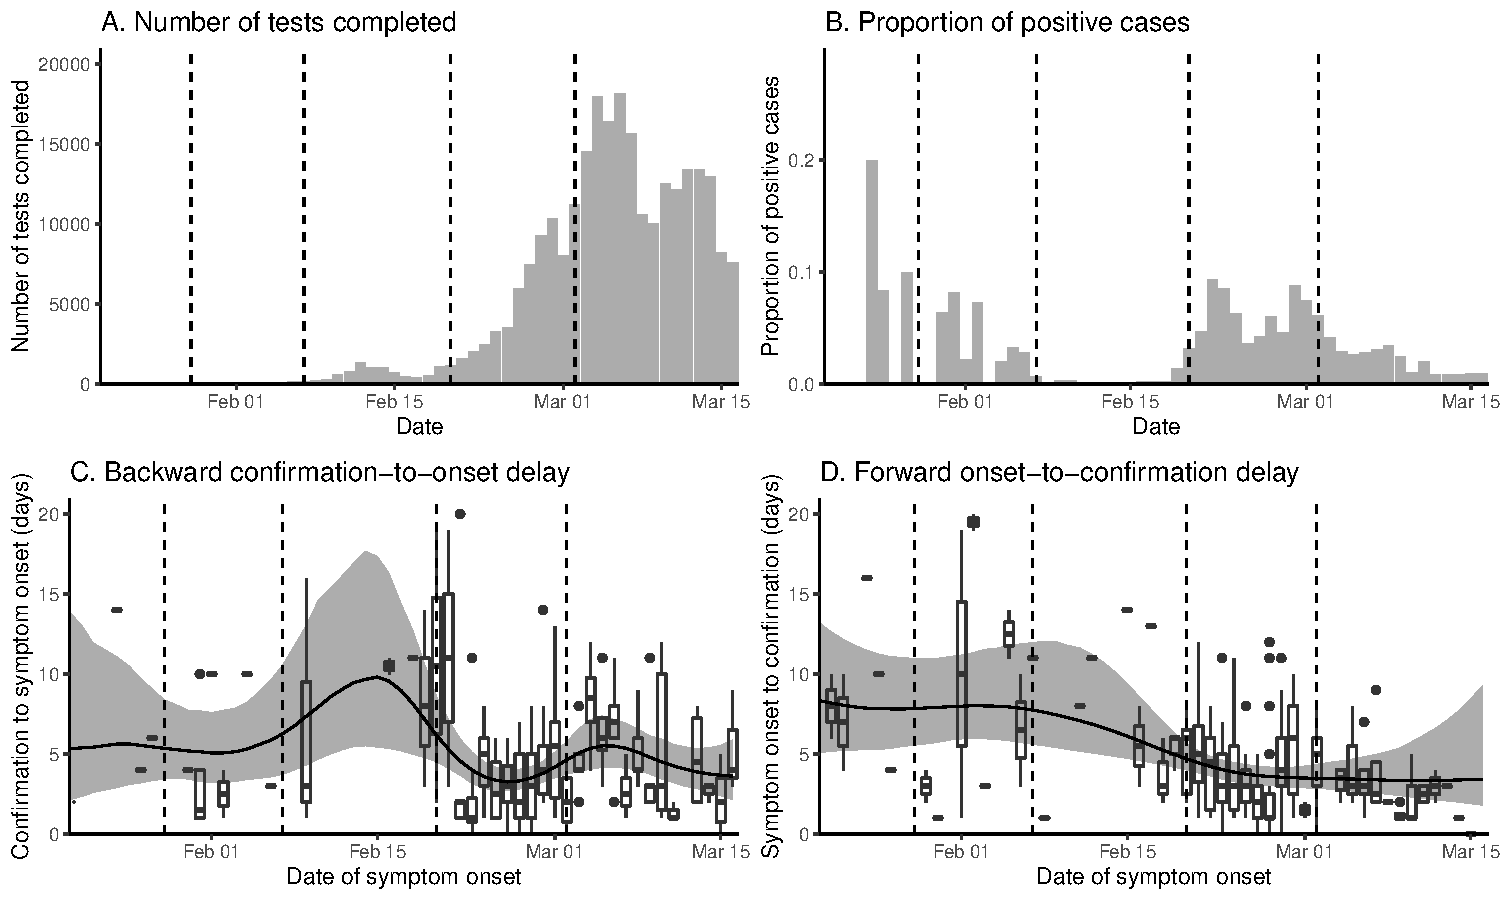
\includegraphics[width=\textwidth]{figure_report_delay.pdf}
\caption{
\textbf{Changes in the number of tests and delay distributions over time.}
}
Vertical lines indicate the date on which testing criteria expanded.
Box plots (C--D) represent the observed delays.
Black lines and gray ribbons represent the median estimates of the mean delays and their associated 95\% credible intervals.
\end{figure}

\pagebreak

\begin{figure}[!ht]
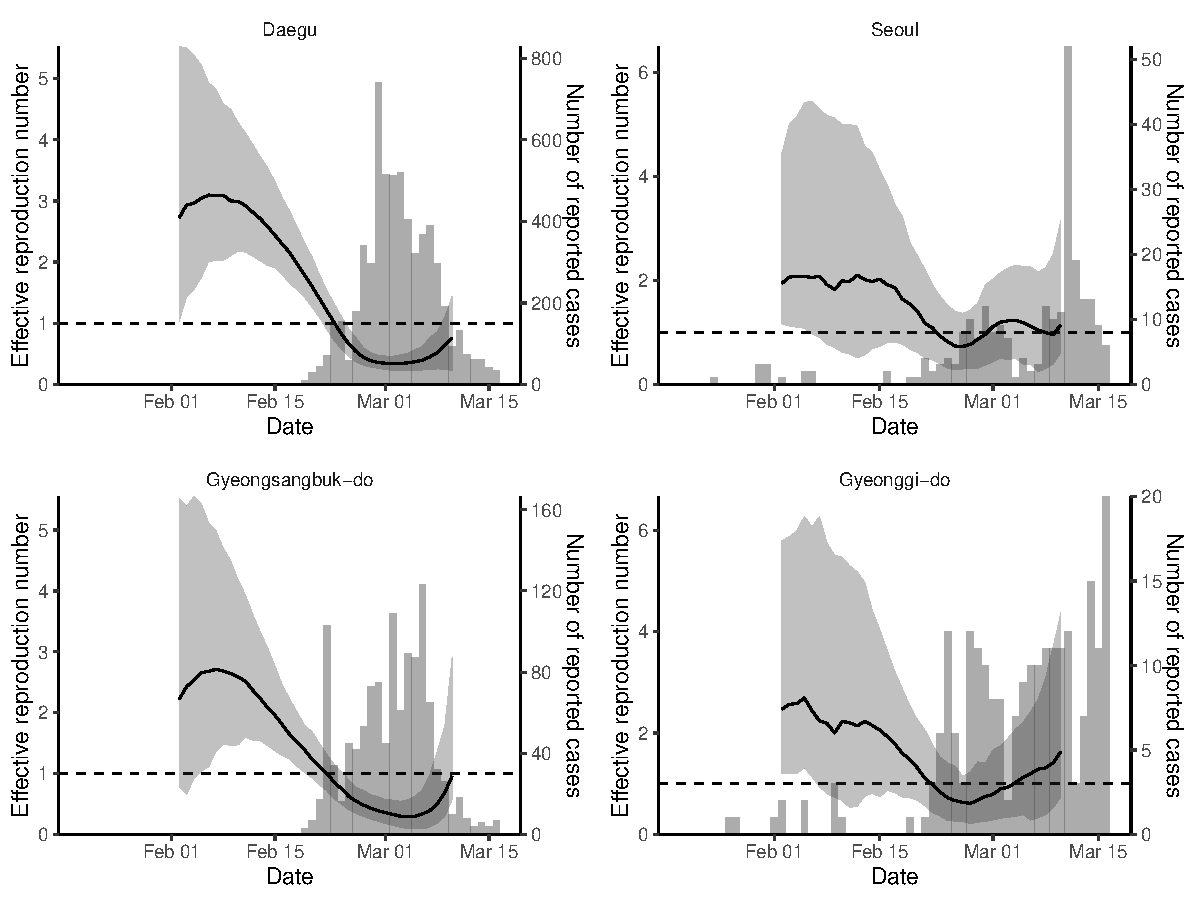
\includegraphics[width=\textwidth]{figure_R_t_all.pdf}
\caption{
\textbf{Comparison of time-dependent reproduction number and the daily number of reported cases in Daegu, Seoul, Gyeongsangbuk-do, and Gyeonggi-do.}
}
\end{figure}

\pagebreak

\begin{figure}[!ht]
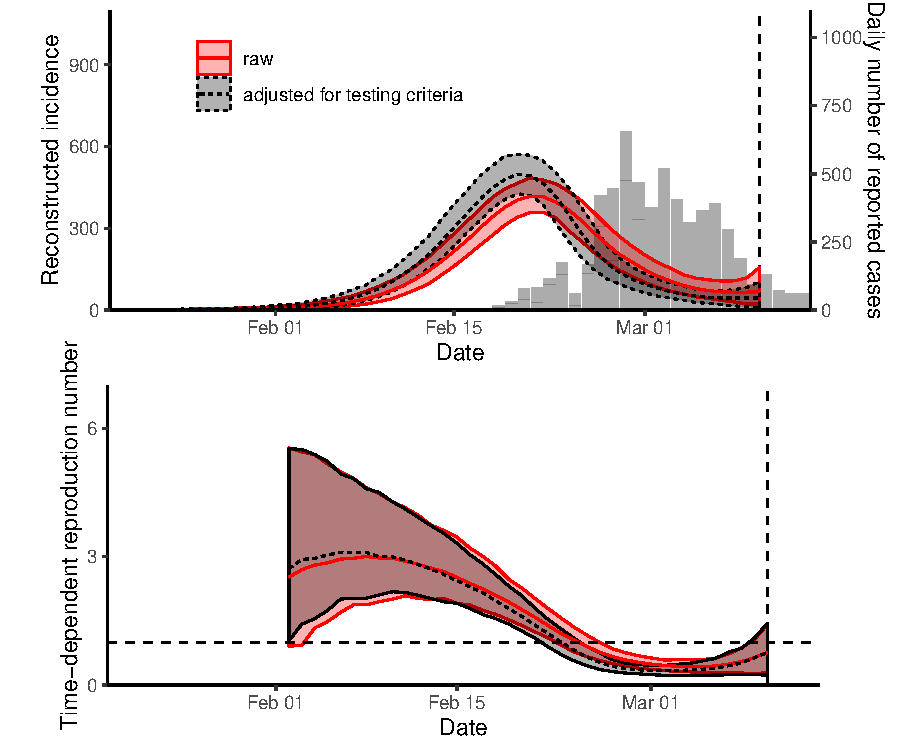
\includegraphics[width=\textwidth]{figure_R_t_daegu.pdf}
\caption{
\textbf{Sensitivity analysis of estimates of $\mathcal R_t$ in Daegu.}
}
\end{figure}

\pagebreak

\begin{figure}[!ht]
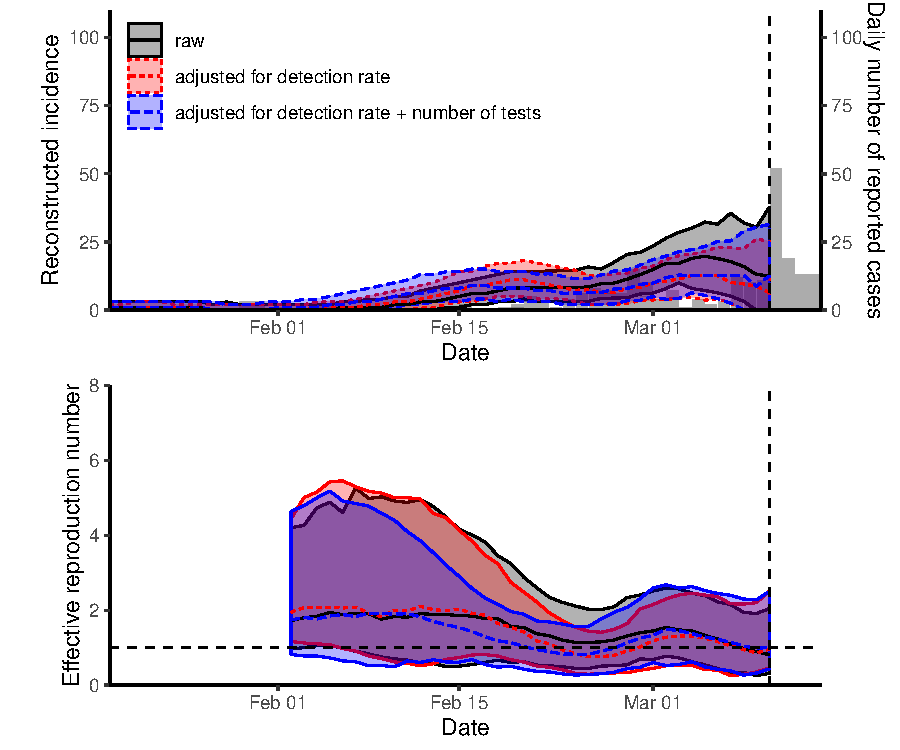
\includegraphics[width=\textwidth]{figure_R_t_seoul.pdf}
\caption{
\textbf{Sensitivity analysis of estimates of $\mathcal R_t$ in Seoul.}
}
\end{figure}

\pagebreak

\begin{figure}[!ht]
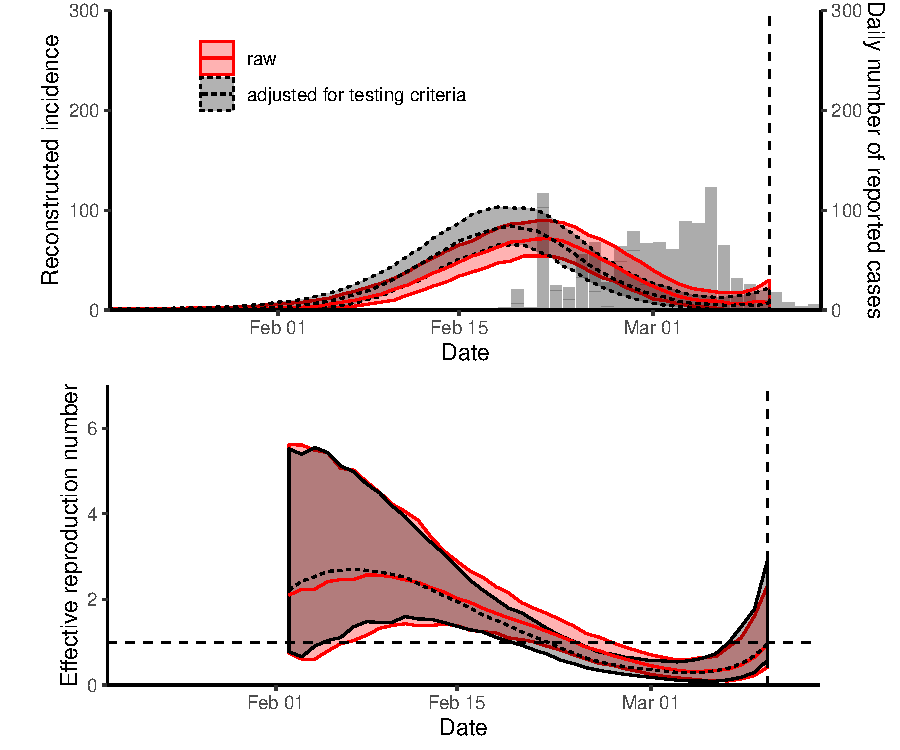
\includegraphics[width=\textwidth]{figure_R_t_gyeongbuk.pdf}
\caption{
\textbf{Sensitivity analysis of estimates of $\mathcal R_t$ in Gyeongsangbuk-do.}
}
\end{figure}

\pagebreak

\begin{figure}[!ht]
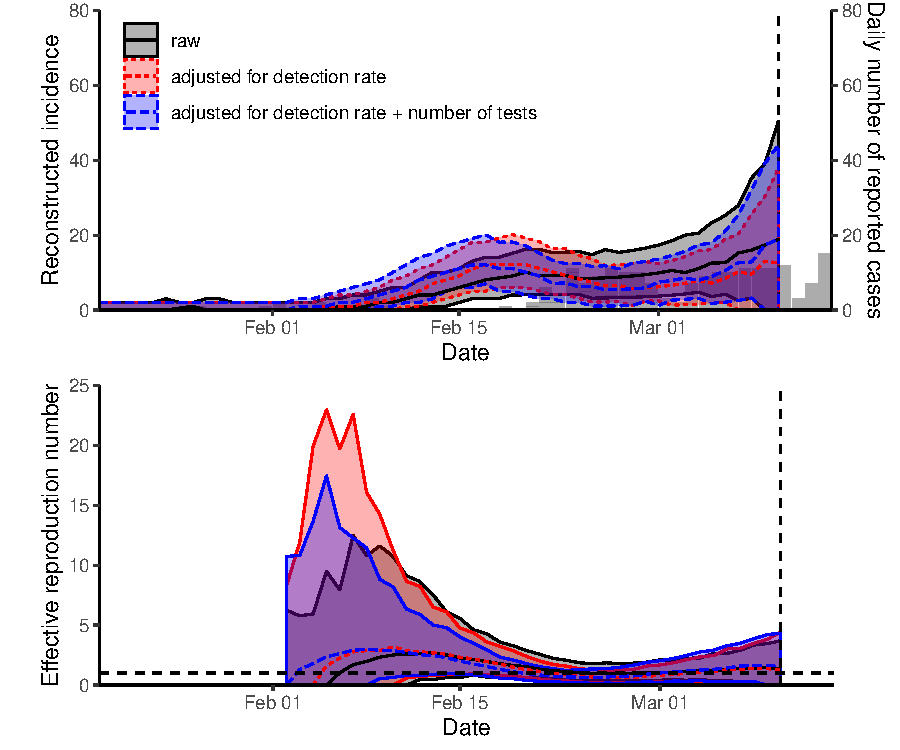
\includegraphics[width=\textwidth]{figure_R_t_gyeonggi.pdf}
\caption{
\textbf{Sensitivity analysis of estimates of $\mathcal R_t$ in Gyeonggi-do.}
}
\end{figure}

\pagebreak

\begin{figure}[!ht]
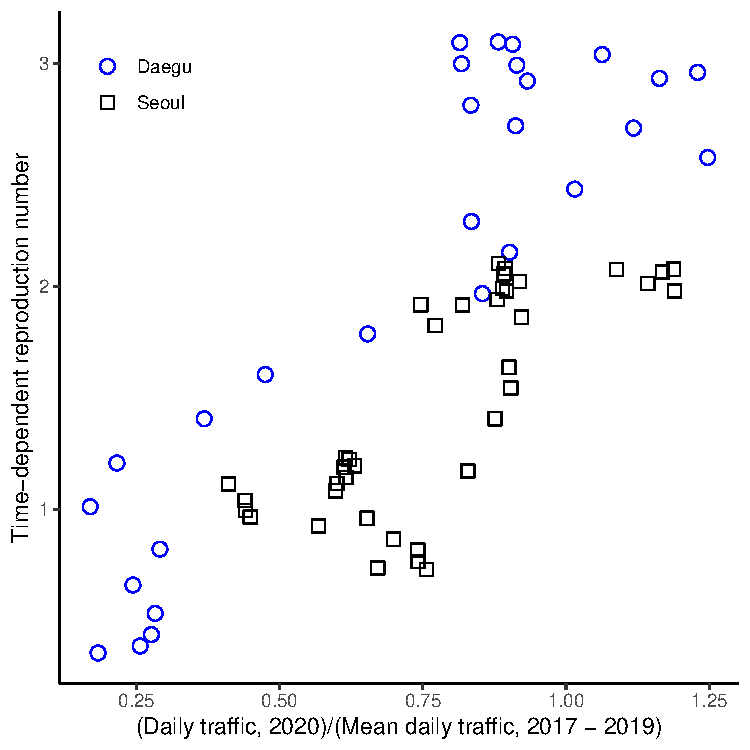
\includegraphics[width=\textwidth]{traffic.pdf}
\caption{
\textbf{Scatter plot of the normalized traffic volume and the median estimates of $\mathcal R_t$.}
}
\end{figure}

\pagebreak

\begin{figure}[!ht]
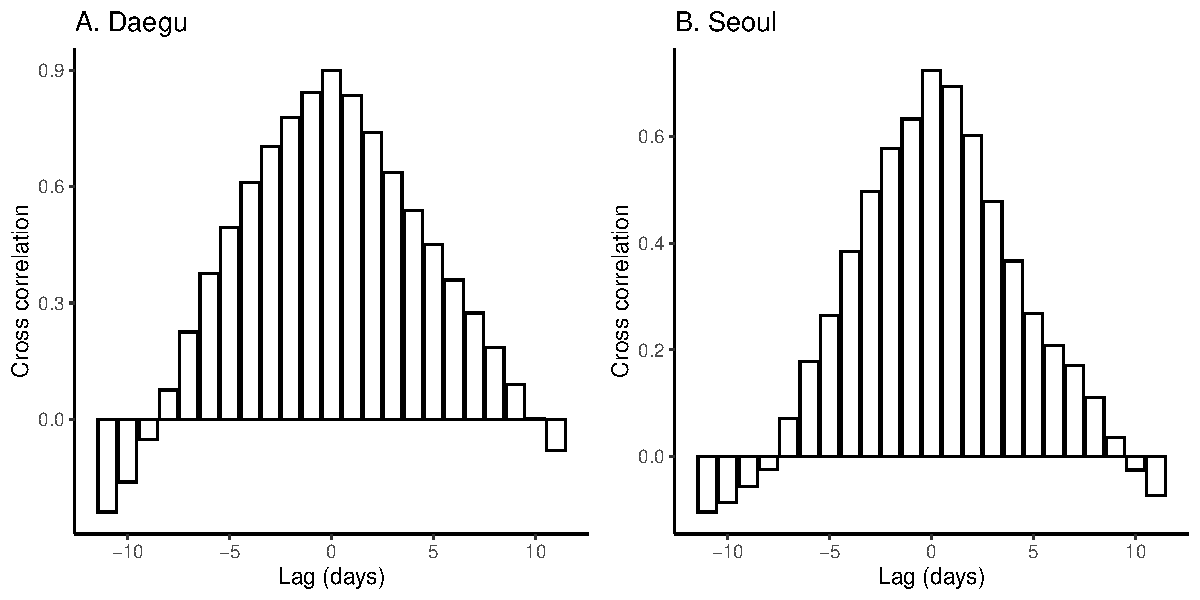
\includegraphics[width=\textwidth]{figure_cross.pdf}
\caption{
\textbf{Cross correlation between the normalized traffic volume and the median estimates of $\mathcal R_t$.}
}
\end{figure}

\pagebreak

\begin{figure}[!ht]
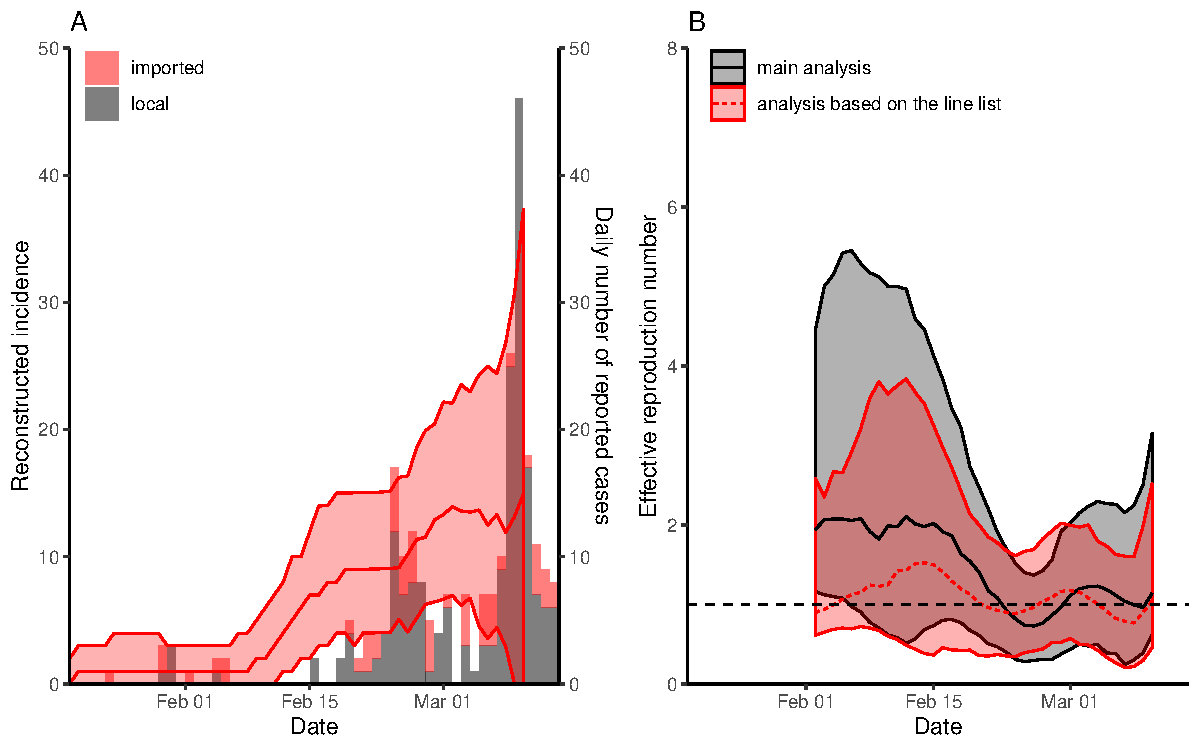
\includegraphics[width=\textwidth]{figure_R_t_seoul_linelist.pdf}
\caption{
\textbf{Comparison of time-dependent reproduction number in Seoul using the number of reported cases by the KCDC and the line list provided by the Seoul Metropolitan Government.}
Using line list, we reconstructed incidence for local $I_t^{\textrm{local}}$ and imported $I_t^{\textrm{imported}}$ cases separately based on the method described in the main text. Then, we estimated the time-dependent reproduction number via $\mathcal R_t = I_t^{\textrm{local}}/\sum_{k=1}^{14} I_{t-k} w_k$, where $I_t=I_t^{\textrm{local}}+I_t^{\textrm{imported}}$. We did not account for changes in testing criteria in this analysis.
The line lists were obtained from \url{http://news.seoul.go.kr/welfare/archives/513105}.
}
\end{figure}
